\begin{document}
The current driver for this lab was created using an MCP6004 op amp. The op amp is to act as the driver for the gate of a 2N3904 Bipolar Junction Transistor (BJT). The generic circuit for the current driver is shown in Figure \ref{fig:currentgeneric}. 
	
	\begin{figure}[H]
		\centering
		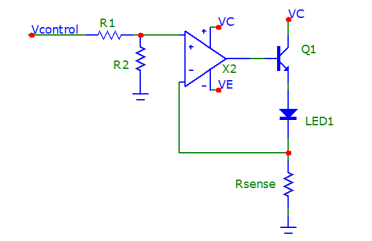
\includegraphics[width=.6\textwidth]{CircuitDevelopment/ledgeneric.png}
		\caption{Generic current driver circuit \cite{b2}}
		\label{fig:currentgeneric}
	\end{figure}

The key to operation of the current driver is the BJT transistor. A BJT transistor, in contrast with the metal oxide semiconducting field effect transistor (MOSFET), is capable of producing current by both types of Charge Carriers. This effectively allows the BJT to behave as a NPN or PNP transistor depending on the size of the input current. This also allows the BJT to use a smaller current signal to control a larger current. 

The operation of a BJT is paramount for this lab. The MCP6004 is only capable of outputing around 20mA of current. The IR LED in use, however, has a forward current of 100mA \cite{LEDDATASHEET}. A much larger current has to generated in order for the LED to operate. 

The MCP6004 is used to set the node voltage for R$_{sense}$. The op amp is assumed to be ideal, so $V_- = V_+$. In order to ensure that the LED is forward biased, the node voltage should be less than the sum of the voltage drops from $V_{supply}$ over the BJT and the diode. The lab briefing \cite{b2} states to set $V_-$ less then 3V.

In order to attain a suitable voltage, a voltage divider is placed at the input to the op amp. The source voltage is the output from the signal conditioner, and was found to be 5V. In order to be less than 3V, a 50/50 voltage divider was used in order to create an input of 2.5V. With this voltage, and the maximum forward current of 200mA, the value for R$_{sense}$ can solved using Ohm's Law. The final value for R$_{sense}$ is 13$\Omega$.

The simulated circuit for current driver is seen in Figure \ref{fig:currentdriverschem}.

%%PICS HERE DAWG
The circuit required no changes from design to simulation. The current through the LED can be seen in Figure \ref{fig:simcurrentlab4}. The simulation was performed using a transient analysis integrated with Matlab.

\begin{figure}
	\centering
	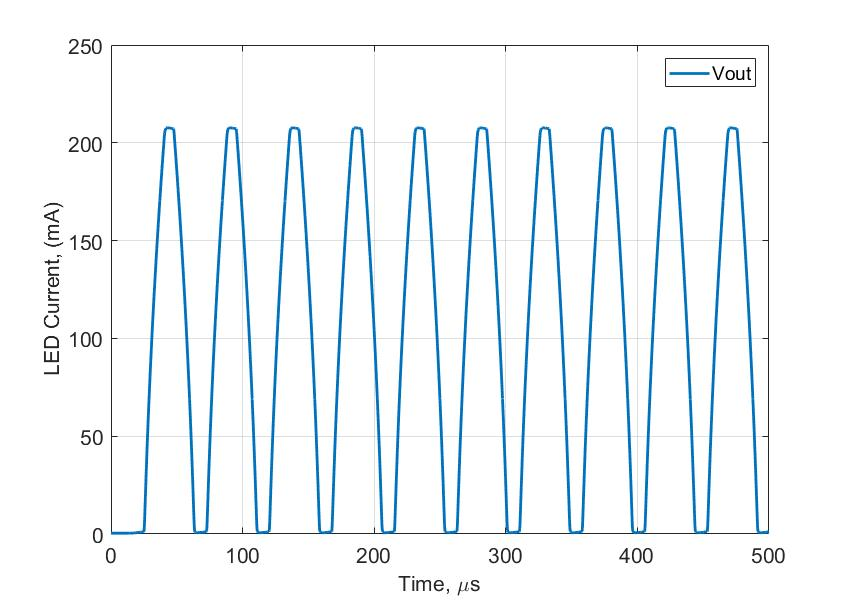
\includegraphics[width=0.7\linewidth]{CircuitDevelopment/sim_current_lab4}
	\caption[Simulated current]{Simulated current through the LED}
	\label{fig:simcurrentlab4}
\end{figure}

The current through the LED matched the calculated value of 200mA



\end{document}